\documentclass[11pt, conference,compsoc]{IEEEtran}

\ifCLASSOPTIONcompsoc
  % IEEE Computer Society needs nocompress option
  % requires cite.sty v4.0 or later (November 2003)
  \usepackage[nocompress]{cite}
\else
  % normal IEEE
  \usepackage{cite}
\fi

\usepackage{graphicx}
\usepackage{tabularx}
\usepackage{amsmath}
\interdisplaylinepenalty=2500

% *** ALIGNMENT PACKAGES ***
%
%\usepackage{array}
% Frank Mittelbach's and David Carlisle's array.sty patches and improves
% the standard LaTeX2e array and tabular environments to provide better
% appearance and additional user controls. As the default LaTeX2e table
% generation code is lacking to the point of almost being broken with
% respect to the quality of the end results, all users are strongly
% advised to use an enhanced (at the very least that provided by array.sty)
% set of table tools. array.sty is already installed on most systems. The
% latest version and documentation can be obtained at:
% http://www.ctan.org/pkg/array

% *** SUBFIGURE PACKAGES ***
%\ifCLASSOPTIONcompsoc
%  \usepackage[caption=false,font=footnotesize,labelfont=sf,textfont=sf]{subfig}
%\else
%  \usepackage[caption=false,font=footnotesize]{subfig}
%\fi
% subfig.sty, written by Steven Douglas Cochran, is the modern replacement
% for subfigure.sty, the latter of which is no longer maintained and is
% incompatible with some LaTeX packages including fixltx2e. However,
% subfig.sty requires and automatically loads Axel Sommerfeldt's caption.sty
% which will override IEEEtran.cls' handling of captions and this will result
% in non-IEEE style figure/table captions. To prevent this problem, be sure
% and invoke subfig.sty's "caption=false" package option (available since
% subfig.sty version 1.3, 2005/06/28) as this is will preserve IEEEtran.cls
% handling of captions.
% Note that the Computer Society format requires a sans serif font rather
% than the serif font used in traditional IEEE formatting and thus the need
% to invoke different subfig.sty package options depending on whether
% compsoc mode has been enabled.
%
% The latest version and documentation of subfig.sty can be obtained at:
% http://www.ctan.org/pkg/subfig




% *** FLOAT PACKAGES ***
%
%\usepackage{fixltx2e}
% fixltx2e, the successor to the earlier fix2col.sty, was written by
% Frank Mittelbach and David Carlisle. This package corrects a few problems
% in the LaTeX2e kernel, the most notable of which is that in current
% LaTeX2e releases, the ordering of single and double column floats is not
% guaranteed to be preserved. Thus, an unpatched LaTeX2e can allow a
% single column figure to be placed prior to an earlier double column
% figure.
% Be aware that LaTeX2e kernels dated 2015 and later have fixltx2e.sty's
% corrections already built into the system in which case a warning will
% be issued if an attempt is made to load fixltx2e.sty as it is no longer
% needed.
% The latest version and documentation can be found at:
% http://www.ctan.org/pkg/fixltx2e


%\usepackage{stfloats}
% stfloats.sty was written by Sigitas Tolusis. This package gives LaTeX2e
% the ability to do double column floats at the bottom of the page as well
% as the top. (e.g., "\begin{figure*}[!b]" is not normally possible in
% LaTeX2e). It also provides a command:
%\fnbelowfloat
% to enable the placement of footnotes below bottom floats (the standard
% LaTeX2e kernel puts them above bottom floats). This is an invasive package
% which rewrites many portions of the LaTeX2e float routines. It may not work
% with other packages that modify the LaTeX2e float routines. The latest
% version and documentation can be obtained at:
% http://www.ctan.org/pkg/stfloats
% Do not use the stfloats baselinefloat ability as the IEEE does not allow
% \baselineskip to stretch. Authors submitting work to the IEEE should note
% that the IEEE rarely uses double column equations and that authors should try
% to avoid such use. Do not be tempted to use the cuted.sty or midfloat.sty
% packages (also by Sigitas Tolusis) as the IEEE does not format its papers in
% such ways.
% Do not attempt to use stfloats with fixltx2e as they are incompatible.
% Instead, use Morten Hogholm'a dblfloatfix which combines the features
% of both fixltx2e and stfloats:
%
% \usepackage{dblfloatfix}
% The latest version can be found at:
% http://www.ctan.org/pkg/dblfloatfix
\usepackage{url}

% correct bad hyphenation here
\hyphenation{op-tical net-works semi-conduc-tor}

\begin{document}

\title{A Study of the Medical Uninsured Rate and its
Impact on the 2016 US Presidential Election at the County Level in the Continental United States}

\author{\IEEEauthorblockN{David Fan}
\IEEEauthorblockA{Case School of Engineering\\
Case Western Reserve University\\
Cleveland, Ohio 44106}
\and
\IEEEauthorblockN{Ted Timbrell}
\IEEEauthorblockA{Case School of Engineering\\
Case Western Reserve University\\
Cleveland, Ohio 44106}}

% make the title area
\maketitle

% As a general rule, do not put math, special symbols or citations
% in the abstract
\begin{abstract}
The 2016 United States Presidential Election and its buildup has led to one of the most divided periods in the country's history. There existed a feeling among some that regardless of who won the election, the Democrat Hillary Clinton or the Republican and eventual victor Donald Trump, the people would be lacking adequate leadership. Most of the polls leading up the election had Donald Trump's chances of victory at slim to none. Following the 2016 election, many have attempted to find explanations for how Donald Trump was able to defeat the political veteran Hillary Clinton. In this paper we explore the potential causal effect of uninsured rate at the county level on the fraction of the county that voted for Donald Trump in the Continental United States. Using county level data from the 2016 US Election and socio-economic county demographic data, we were able to use \textbf{Stabilized Inverse Probability Weighting} to fit a \textbf{Quadratic Marginal Structural Model}. We found that at the mean level of county uninsured rate, uninsured rate had an estimated marginal causal effect of ($0.1316 \pm 0.2643$). We then fit an outcome regression model which agreed with the result of the previous method. Thus, we cannot conclude that for a county with the average uninsured rate, uninsured rate had any causal effect on the way the county voted in the 2016 US Presidential Election.
\end{abstract}


\section{Introduction}
% no \IEEEPARstart
In 2017, a study conducted by the Pew Research Center found that Americans were more divided along party lines than ever before \cite{pewdivided}. This is hardly surprising as the year before saw one of the most controversial United States presidential elections of modern history. With President Barack Obama finishing his second term, 2016 would see a new president take power. There were two main challengers for the Democratic Party nomination: veteran Democrat Hillary Clinton and progressive independent Bernie Sanders. Following a controversial \cite{DNCcontroversy} primary, Hillary Clinton was eventually nominated to be the Democratic Party's nominee. The Republican field began with numerous candidates with high potential. These included Ohio Governor John Kasich, Florida Senator Marco Rubio, and Texas Senator Ted Cruz among notable business executives and a neurosurgeon \cite{RNCprimary}. Despite what many believed to initially be a publicity stunt, Donald Trump eventually rose above the field to claim the Republican party nomination \cite{538}. Trump rose on a populist and nationalist message, claiming to champion the "forgotten men and women of America" \cite{forgotten}. The inflammatory rhetoric of Trump continued on throughout the campaign season, drawing the ire of many critics. He faced criticisms for quotes likening Mexicans to criminals and rapists, for promising to build a wall on the Mexican-American border, and for expressing a desire to ban all Muslims from the country \cite{controversy}. While Hillary Clinton had her share of campaign controversies, including her usage of a private email server during her tenure as Secretary of State in the Obama Administration and for infamously saying that half of Trump's supporters belong in a "basket of deplorables" \cite{deplorable}, she was strongly favored by polls to become the next President of the United States \cite{polls}.

After Trump's victory, many sought to attempt to explain how he outperformed his polling results and how no one predicted his victory. Some credited his victory to the spread of fake news on social media sites, some blamed Hillary Clinton for being what they perceived as a weak candidate, and some believed that it was likely that people were ashamed to respond to polls with their true beliefs. Whether one of these reasons, a combination of these reasons, or an entirely different reason involving Russia and Russian President Vladimir Putin \cite{Russia} were the reason for Trump's victory, it now presents an interesting case study for many political scientists and for those studying causal effects.

In this paper we are attempting to study any potential causal effect that the percentage of people in a county that lack health insurance had on the way that county voted in the 2016 United States presidential election. Health care in the last twenty years has been an incredibly contentious topic. This amplified with the passing of the Affordable Care Act in 2010 under President Obama. The Affordable Care Act was passed in an effort to reduce the number of people without health insurance. It did this by implementing an individual mandate that everyone be covered by health insurance. The unpopular nature of the tax associated with the individual mandate, coupled with efforts to reduce the number of uninsured people raises the question of how the effort turned out politically. The bill has become a large target for the Republican Party, with prominent Republicans including President Trump calling it \textit{"Obamacare"} rather than its official name to tie its popularity to the popularity of President Obama and, indirectly, the Democratic Party. Health care was a hot topic during the 2016 Presidential Debates, with many seeing it as a core policy in both candidate's platforms. Investigating the causal effect that actual uninsured rates had on voting results may shed some light into the complicated 2016 election and its aftermath.

\section{Problem Description}
To analyze the causal effect that the percentage of people in a county that lack health insurance had on the way that county voted in the 2016 United States presidential election, we need to take county level data for voting history and socio-economic trends and appropriately note confounders so that we can adjust for them to remove bias in our methodology. 

\subsection{Dataset}
The dataset we are using was originally assembled by Emil O. W. Kirkegaard in his paper "Inequality across US counties: an S factor analysis". The dataset can be found at \url{https://github.com/Deleetdk/USA.county.data}. In the process of this study we have trimmed down number of variables used in the set. This is due in part because the data didn't end up being relevant to the analysis, and due to a lack of trust in the author of the dataset. 

After beginning this body of work, we discovered more about the author of the dataset, Kirkegaard. It seems that he's an individual that uses science and math to justify very controversial and, in our view, unacceptable ideas. To avoid giving him more undue exposure, we will not go into further detail about the views that he holds or the numerous controversies involving him, but more information can be found with even the most cursory Internet search. While it is regrettable that we did not discover the author of the dataset's background early into our work, we were able to verify that the integrity of the data was not compromised. Any fields that were added by the author himself, such as the "S factor," were removed. Other fields that were superfluous to this problem, such as longitude and latitude, were also removed.

This particular dataset was advantageous because it combined data for US counties $(N\approx 3,100)$ from a variety of reputable sources. The first being Measure of America's county data, which contains data on demographics of each county as well as several socio-economic variables. That dataset can be found at \url{http://www.measureofamerica.org/download-agreement/}. The second from County Health rankings, an organization sponsored by the University of Wisconsin's Population Health Institute. This set contains data on health outcomes and is the source of our uninsured rate measure. It can be found at \url{http://www.countyhealthrankings.org/rankings/data}. The third and fourth were eventually trimmed from our final version of the dataset, although they contained geographic, age, and gender information from the US Census. They can be found at \url{http://factfinder.census.gov/bkmk/table/1.0/en/DEC/10_SF1/G001/0100000US.05000.003} and \url{http://factfinder.census.gov/bkmk/table/1.0/en/ACS/10_5YR/S0101/0100000US.05000.003}. The fifth was also trimmed from the final dataset, but it contained climate data from the National Oceanic and Atmospheric Administration. For reference, the dataset can be found at \url{http://www.ncdc.noaa.gov/cdo-web/datatools/normals}. The sixth dataset contained data on education but ended up being redundant for our purposes with the data gathered from the set from Measure of America. The source for the sixth dataset has seemingly shut down so using variables and values from that set would have been inadvisable. The election data was originally reported by the Associated Press through the week of Nov. 8, 2016 and displayed on an interactive web page by the New York Times. The page can be found at \url{https://www.nytimes.com/elections/results/president}. To create his original dataset, the author simply joined those datasets based on county id (scraping websites for the data where necessary). As mentioned above, in our version of the dataset, we ended up removing many variables.

Although it was helpful to have the set compiled for us, there were some anomalies in the dataset that we had to account for. The first is that Shannon County was listed as two separate counties because of a name change in between the 2012 and 2016 election cycle. The county is now named Oglala Lakota County. Data for the two entries was easily merged as there was no overlap in fields. The second was Bedford City Virgina. The city used to be independent and was previously categorized separately but in 2013 it incorporated into the county of Bedford. Since that makes the entry for Bedford City outdated, it was discarded. The third and most odd problem we ran into is that Alaska doesn't actually have counties. Although there could be an argument to censor the state because it is known for its unique challenges when it comes to insurance and health care, we removed the values because we wanted to stick with relatively standard county level data. Due to the borough system, many of the Alaskan areas weren't included in the original datasets. As a result of these facts, Alaska isn't included in this study. This realization led us to conclude that defining the scope of the problem to the Continental United States would yield more conclusive and interpretable results.

\subsection{Causal Graph}
\begin{figure*} 
	\centering
	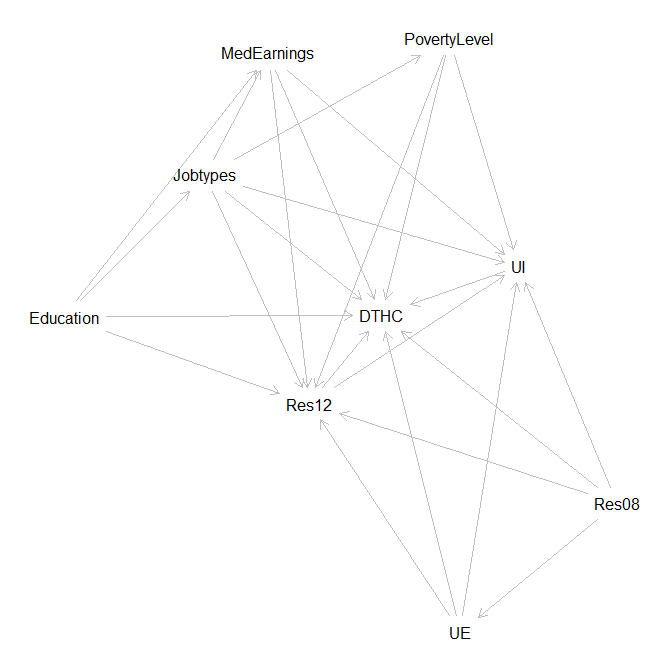
\includegraphics[width=.7\textwidth]{dag}
	\caption{Causal Graph Representing the Causal Relationships between Socio-economic County Data and Voting History}
    \label{dag}
\end{figure*}
Like most observational studies, this problem contains many confounding variables. In this next section we are going to justify our decisions of causality between these variables. Starting simply, our primary goal is to estimate or see any potential causal effect from the uninsured rate variable \textbf{UI}, measured in 2014, to the variable \textbf{DTHC} of the voting percentages for the democratic and republican candidates the 2016 presidential elections. 

The uninsured rate \textbf{UI} only causally affects the 2016 election outcome \textbf{DTHC} as it was measured after the 2008 and the 2012 elections. There are no other significant variables that \textbf{UI} causally affects in our problem. The outcome of the 2016 election doesn't causally affect any of the other variables due to it occurring after the other values were recorded.

Our \textbf{Education} variable is actually a combination of several similar confounding variables. It is made up of the percentage of the population with less than a high school diploma, at least a high school diploma, and with at least a bachelor’s degree. These values were all recorded at the same time, and all causally affected the same variables and were causally affected by the same variables. In this case we argue that the \textbf{Education} variable impacts the \textbf{Jobtypes} variable, as traditionally jobs that require higher or lower education are located in areas with access to those employees. Therefore, the education level of the county has a direct causal effect on the type of jobs available in the county. It also impacts the median earnings, denoted \textbf{MedEarnings}, for a county, as higher educated people are typically afforded higher salaries than people with a lower level of education in a job. Finally, we claim that the education level impacts all of the election variables after 2010, the time of its recording, as education levels generally impact values and preferences people might have for political candidates. A large part of political platforms for US Presidential candidates is always education. We argue one's own education level will cause one to prefer one candidate over another based in part on their education platform.

The \textbf{Jobtypes} variable, signifying the types of jobs in a county, is quite similar to \textbf{Education} in that it is really bundle of interrelated values that have identical causal relationships. Each of the values is a job category that is a percentage of the total jobs in that county. The categories are management and related occupations, service occupations, sales and office occupations, farming, fishing and forestry occupations, construction, extraction, maintenance and repair occupations, and finally production, transportation and material moving occupations. \textbf{Jobtypes} was recorded in 2009-2010, so we say that it impacts all election variables after that year simply due to political policy. It also directly affects the median earnings for a county as some jobs are inherently better paid or more in demand and it impacts \textbf{PovertyLevel}, the fraction of the county's population that is at or below the federal poverty level, for the same reason. \textbf{Jobtypes} directly impacts the uninsured rate because job types are sensitive to employer benefits.

The median earnings of a county, which we previously defined as the \textbf{MedEarnings} variable, is simply the real valued median earnings of the residents in that county recorded in 2010. We argue that the median earnings of a county impacts the uninsured rate as income level directly affects the ability for residents to be able to afford insurance policies. It impacts the future elections results as people vote with some form of self-interest and the economy is central to most political platforms.  Although it seems like it should be causation, we argue that \textbf{PovertyLevel} is associated with median earnings and simply shares confounding variables.

\textbf{Res08} is the combined representation of two variables containing the fraction of the total votes for the candidate’s party in each county for the 2008 presidential election. Because these two variables were recorded before most of the other data and the results have such a strong impact on government functioning during this time it tends to connect most other variables. The result of this election impacts future elections and unemployment rate due to government fiscal policy. The uninsured rate is also affected because of expectation and new laws governing health care. 

\textbf{Res12} is the combined representation of two variables containing the fraction of the votes cast for the different candidates in the 2012 presidential election. Due to the time and impact of these results it only affects \textbf{UI}, as it guaranteed the continued existence of the Affordable Care Act, and the \textbf{DTHC} 2016 election results, as it impacts political climate and that there is no incumbent candidate.

The unemployment rate, which we define as \textbf{UE}, was collected in 2010. From this we say that it impacts the next two elections \textbf{DTHC} and \textbf{Res12} for clear economic reasons, as well as \textbf{UI} due to the reliance on jobs for health insurance in America.

\section{Methodology}
To measure the existence of a causal effect from our problem we have to deal with a couple key issues. First, that we have a high number of confounding variables. Second, that our treatment, outcome, and covariates are all continuous. This prevents us from using simple methods that work well in binary or discrete settings. Instead we will first use stabilized inverse probability weighting to then fit a marginal structured model and later an outcome regression method.
\subsection{Inverse Probability Weighting}
Inverse probability weighting's primary benefit is that it allows us to adjust for confounding variables. We can define the average causal effect (\textbf{ACE}) as $E[Y^{a}]-E[Y^{a=0}]$ at a certain value of a. The average associational difference, $E[Y|a]- E[Y|a=0]$, isn't guaranteed to be the same because of confounding variables. These variables might affect the population that end up with different treatment values. Inverse probability weighting adjusts for this by creating pseudo populations in which the causal effect of the confounders on the treatment is removed \cite{hernan}. These pseudo populations are weighted by the likelihood of the treatment given the values of the confounding variables (See \ref{weights}).
\begin{equation}
\label{weights}
W^A = \frac{1}{f(A|L)}
\end{equation} 
\begin{equation}
f(A|L) = P[A=a|L]
\end{equation}
In the case of a continuous treatment this likelihood is modeled as a Gaussian distribution with mean $\mu_L = E[A|L]$ and variance of residuals $\sigma^2$ for all combinations of L \cite{hernan}. Additionally, because our treatment is continuous we must stabilize our weights. Stabilized IP Weights can be calculated using the following formula:
\begin{equation}
W^A = \frac{f(A)}{f(A|L)}
\end{equation}
where $f(A)$, the stabilizing factor, is the probability density function of the treatment. The numerator of the stabilized weights can be calculated by fitting A to a Gaussian distribution. The denominator of the stabilized weights can be calculated by fitting a logistic regression.

To determine the average causal difference, the stabilized IP weights are then used to fit a quadratic marginal structural model as shown in \ref{msm}.
\begin{equation}
\label{msm}
E[Y^{a}] = \beta_0 + \beta_1a + \beta_2a^2
\end{equation}
In our marginal structural model, $\beta_0$ represents the average fraction of a county voting for Trump in 2016 under $a = 0$, or total medical insurance in the county. In other words:
\begin{equation}
\beta_0 = E[Y^{a=0}]
\end{equation}
So we can rearrange \ref{msm} to get a formula for calculating the average causal effect at a certain level of treatment:
\begin{equation}
\label{msmACE}
E[Y^a]-E[Y^{a=0}] = \beta_1a + \beta_2a^2
\end{equation}
To find the parameters $\beta_0$, $\beta_1$, and $\beta_2$, we fit the associational model:
\begin{equation}
E[Y|A] = \theta_0 + \theta_1A + \theta_2A^2
\end{equation}
By fitting the parameters of the associational model, we are able to produce a consistent estimator for the parameters of the marginal structural model.

The calculation of IP weighting and the quadratic marginal structural model is assisted by two R packages. One is the package 'ipw' which runs our IP weighting, and the second is 'survey' which helps with statistics and finding the confidence intervals of our model.
\subsection{Outcome Regression}
To confirm the results of the previous methodology we opted to use outcome regression. Outcome regression is a commonly used parametric tool for causal inference. Normally, structural nested models include parameters for product terms between the treatment and confounders, but not terms for the confounders themselves \cite{hernan}. If we can specify the L-Y association within levels of A, we have the following structural model:
\begin{equation}
E[Y^{a}|L]=\beta_0+\beta_1a+\beta_2aL+\beta_3L
\end{equation}
where $\beta_2$ and $\beta_3$ are vector parameters. The average causal effect of the treatment A on the outcome Y in each stratum of L is then a function of $\beta_1$ and $\beta_2$ while the mean counterfactual outcomes under no treatment in each stratum of L is a function of $\beta_0$ and $\beta_3$ \cite{hernan}. The parameters of the structural model can be estimated by using ordinary least squares to fit the outcome regression model:
\begin{equation}
E[Y|A, C=0, L]=\alpha_0+\alpha_1A+\alpha_2AL+\alpha_3L
\end{equation}
The outcome regression model can then be used to compare the conditional mean estimates.

To simplify the above model, it is common to assume no effect modification by any confounder \cite{hernan}. This eliminates all product terms in the model and simplifies the model into a linear equation:
\begin{equation}
E[Y|A, C=0, L]=\alpha_0+\alpha_1A+\alpha_2L
\end{equation}
In this simplified model, $\alpha_1$ can be interpreted as the average causal effect of treatment. Because there was no censoring in our data, conditioning on $c=0$ is redundant so our final model was:
\begin{equation}
\label{outcome_regression_model}
E[Y|A, L]=\alpha_0+\alpha_1A+\alpha_2L
\end{equation}
Where $Y$ is the fraction of voters in a county that voted Trump in 2016, $A$ is the uninsured rate in the county, and $L$ is all of the confounders defined in our causal graph. The $\alpha_2L$ term is actually the sum of terms for each individual confounder.

\section{Results}
In the following section we will go over the results of our modeling. We first discuss the results of estimating our marginal structural model using stabilized inverse probability weighting. We then discuss the results of our outcome regression model and check if it agrees with the results of our marginal structural model.
\subsection{Stabilized Inverse Probability Weighting and Marginal Structural Model}
\begin{figure} 
	\centering
	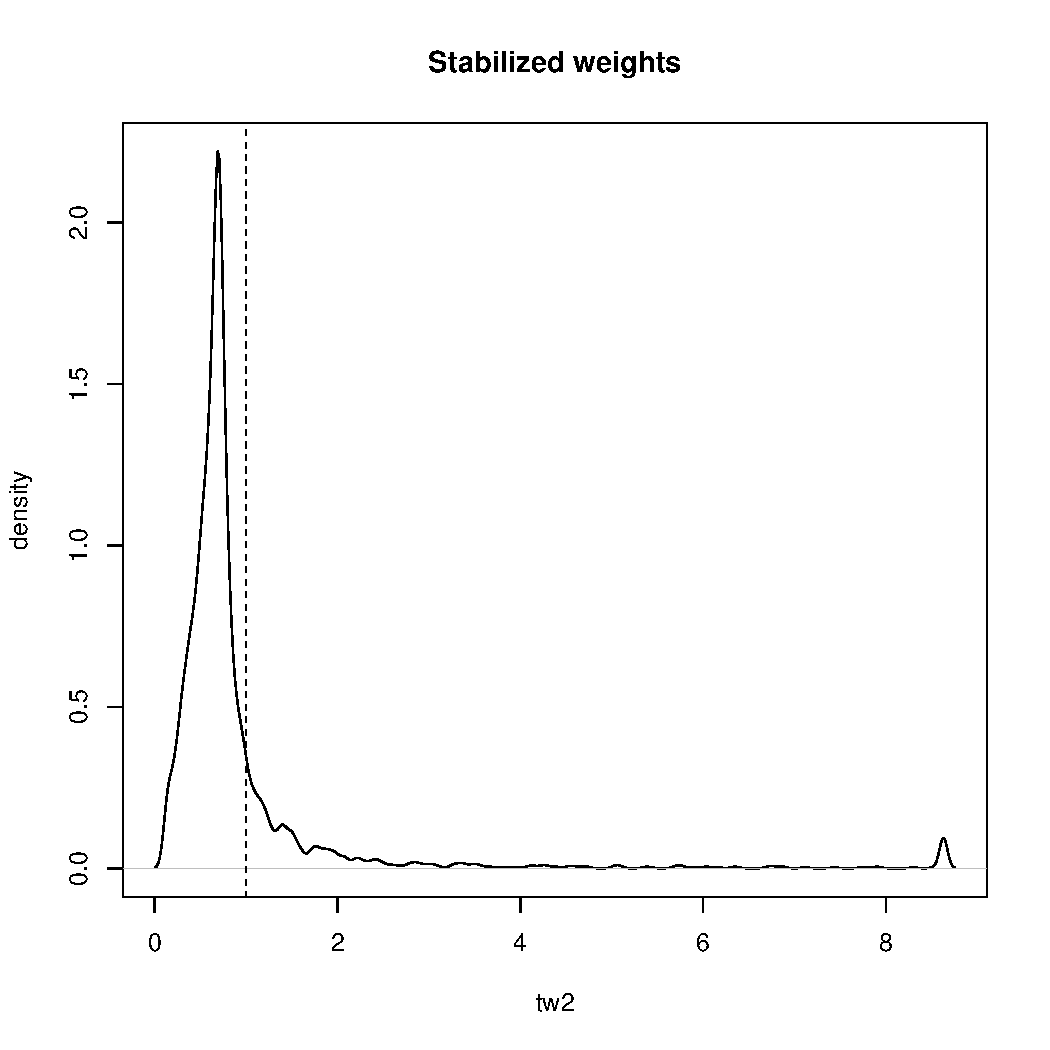
\includegraphics[width=.5\textwidth]{weights}
	\caption{Distribution of Stabilized IP Weights}
    \label{figweights}
\end{figure}
We were able to obtain good results for our stabilized IP Weights. We truncated the weights at 1\% to remove extrema. The resulting distribution can be seen in Figure \ref{figweights}. Table \ref{ipwtable} reports the statistics for the distribution of the truncated IP Weights. As expected with stabilized IP weighting, the mean is close to 1. It seems that there was another point of extrema towards the max end of the IP weight distribution though, so that seems to be pushing the mean closer to 1. Prior to truncating, the max extrema was so large (66298.34) that it pushed the mean to 22.85. This drove the decision to truncate at 1\%.

\begin{table}
\caption{Statistics for the Stabilized IP Weights}
\label{ipwtable}
\begin{center}
\begin{tabular}{ |c |c| c |c|c|c|}
\hline
Min. & 1st Quar. &Median & Mean & 3rd Quar. & Max\\ \hline
0.1289 &0.5257 & 0.6884 & 0.9098 & 0.8373 & 8.6313  \\ \hline
\end{tabular}
\end{center}
\end{table}

In Table \ref{msmtable} we can see the initial output of our estimator for the quadratic marginal structural model and in Table \ref{cimsm} we can see the related confidence intervals for these values. Using our coefficient values and Equation \ref{msmACE}, we found that at the mean level of county uninsured rate, uninsured rate had an estimated marginal causal effect of $(0.1316\pm0.2643)$. As we can see, the bound contains the zero value, and as such we cannot conclude that there the uninsured rate in a county is a causal effect on the way that the county voted in 2016.

\begin{table}
\caption{Coefficients of the marginal structural model}
\label{msmtable}
\begin{center}
\begin{tabular}{ |c |c| c |}
\hline
$(Intercept)$&$Uninsured$&$Uninsured^2$\\ \hline
40.5346133 &1.6432150 &-5.0697341  \\ \hline
\end{tabular}
\end{center}
\end{table}

\begin{table}
\begin{center}
\caption{Confidence Intervals of the marginal structural model}
\label{cimsm}
\begin{tabular}{ |l |c| c |}
\hline
& 2.5 \% &97.5 \% \\  \hline
$(Intercept)$&0.4161592&0.6530675 \\ \hline
$Uninsured$&0.3022877&2.9841422 \\ \hline
$Uninsured^2$&-8.6416134&-1.4978548 \\\hline
\end{tabular}
\end{center}
\end{table}

Furthermore, in Figure \ref{residuals} we can see the plotting of the residuals versus the predicted data of our marginal structural model. We can see that the fit works relatively well at lower predicted values but at higher ones, especially those where Donald Trump won higher percentages of the vote, we see a lot of grouping and a much higher variance from the fit.

We also plotted the dose response curve in Figure \ref{dose-response}. From this we can see the average causal effect vs treatment curve that our marginal structural model fitted and the true values from the uninsured rate to the fraction of the country that voted for Donald Trump. We can see from this that the dose does vary in effectiveness, with the first response being to increase the strength of the outcome, but falling off later. 

\begin{figure} 
	\centering
	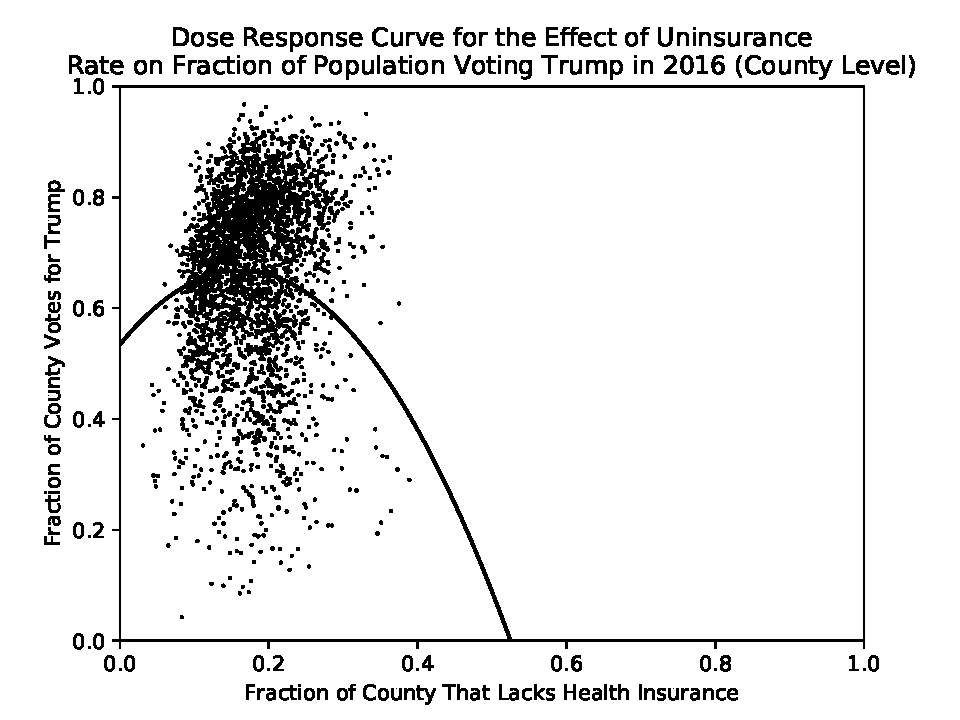
\includegraphics[width=.5\textwidth]{dose-response-scatter}
	\caption{Dose Response Curve of the Effect of Uninsured on Fraction of the Vote Donald Trump Received}
    \label{dose-response}
\end{figure}
\begin{figure} 
	\centering
	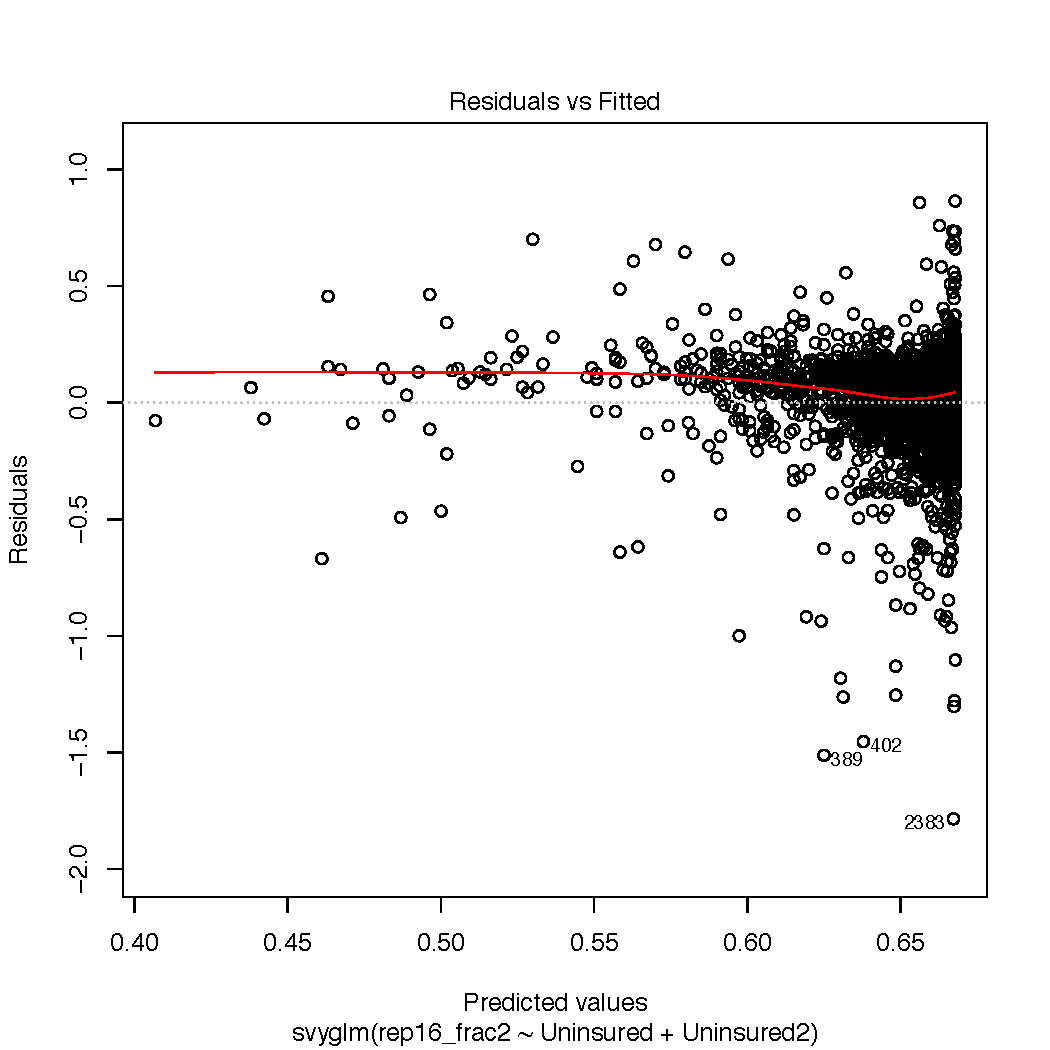
\includegraphics[width=.5\textwidth]{MSM_Residuals}
	\caption{Residuals of the fitted marginal structural model}
    \label{residuals}
\end{figure}
  

\subsection{Outcome Regression}

\begin{table}
\begin{center}
\caption{Coefficients of the linear model}
\label{coefflm}
\begin{tabular}{ |l |c| c |}
\hline
(Intercept)& 1.000000e+00 \\ \hline
dem16\_frac2 &-1.000000e+00  \\ \hline
dem08\_frac2 &5.240273e-11 \\ \hline
dem12\_frac2 &-3.081619e-10 \\ \hline
rep08\_frac2 &NA \\ \hline
rep12\_frac2 &NA \\ \hline
LessThanHighSchool &4.001863e-12 \\ \hline
AtLeastHighSchoolDiploma &2.484397e-12 \\ \hline
AtLeastBachelorsDegree &-3.682953e-13 \\ \hline
MedianEarnings2010dollars &-1.118810e-15 \\ \hline
PovertyRatebelowfederalpovertythreshold &-1.456793e-12 \\ \hline
Management[...]occupations &-6.758984e-11 \\ \hline
Serviceoccupations &-6.773471e-11 \\ \hline
Salesandofficeoccupations &-6.815968e-11 \\ \hline
Farmingfishingandforestryoccupations &-6.484763e-11 \\ \hline 
Constructione[...]ccupations &-6.750469e-11\\ \hline 
Productiontrans[...]occupations &-6.715159e-11 \\ \hline
Uninsured &-1.783708e-10 \\ \hline
Unemployment &1.035804e-10\\ \hline
\end{tabular}
\end{center}
\end{table}

\begin{table*}
\begin{center}
\caption{Confidence Intervals of the linear model}
\label{conflm}
\begin{tabularx}{.7\textwidth}{ |X|c|c|}
\hline
 &2.5 \%& 97.5 \% \\ \hline
(Intercept)&1.000000e+00 &1.000000e+00 \\ \hline 
dem16\_frac2&-1.000000e+00 & 1.000000e+00 \\ \hline 
dem08\_frac2 &-3.543460e-10 & 4.591515e-10 \\ \hline 
dem12\_frac2 & -8.426581e-10 & 2.263343e-10 \\ \hline 
rep08\_frac2 &NA &           NA \\ \hline 
rep12\_frac2&NA &           NA \\ \hline 
LessThanHighSchool &-2.509907e-12 & 1.051363e-11 \\ \hline 
AtLeastHighSchoolDiploma &-3.667854e-12 & 8.636647e-12 \\ \hline 
AtLeastBachelorsDegree &-3.398741e-12 & 2.662150e-12 \\ \hline 
MedianEarnings2010dollars &-4.796302e-15 & 2.558682e-15 \\ \hline 
PovertyRatebelowfederalpovertythreshold& -4.721032e-12 & 1.807446e-12 \\ \hline 
Managementprofessionalandrelatedoccupations &-2.770800e-10 & 1.419003e-10 \\ \hline 
Serviceoccupations  &-2.772484e-10 & 1.417790e-10 \\ \hline 
Salesandofficeoccupations    &-2.775478e-10 & 1.412285e-10 \\ \hline 
Farmingfishingandforestryoccupations  & -2.743314e-10 & 1.446361e-10 \\ \hline 
Construction...occupations&-2.769987e-10 & 1.419893e-10 \\ \hline 
Production...occupations &-2.766484e-10 & 1.423452e-10 \\ \hline 
Uninsured    &-4.954239e-10 & 1.386822e-10 \\ \hline 
Unemployment   &-3.991104e-10 & 6.062712e-10 \\ \hline 
\end{tabularx}
\end{center}
\end{table*}
We fit our outcome regression model to the data, and Table \ref{coefflm} displays the coefficients of the fit while Table \ref{conflm} contains the confidence intervals for each coefficient. In Figure \ref{outcome-regression} we can see the residuals of our regression model. We see that aside from a string of parallel outliers we find a pretty strong adherence to our fit. As mentioned in the methods section, in our simplified outcome regression model (Equation \ref{outcome_regression_model}), the coefficient of the treatment can be interpreted as the average causal effect of the treatment on the outcome. From our fit, we find an average causal effect of  $(-1.783708e-10\pm3.1705305e-10)$. As $0$ is included within our confidence interval, the outcome regression cannot conclude that there exists a causal effect of the treatment on the outcome. This agrees with the result of the previous method.

One thing of interest to point out is the "NA" results for both \textbf{rep08\_frac2} and \textbf{rep12\_frac2}. This was likely due the fact that those two variables are equivalent to one minus their \textbf{dem0X\_frac2} counterparts so they're directly dependent.
\begin{figure} 
	\centering
	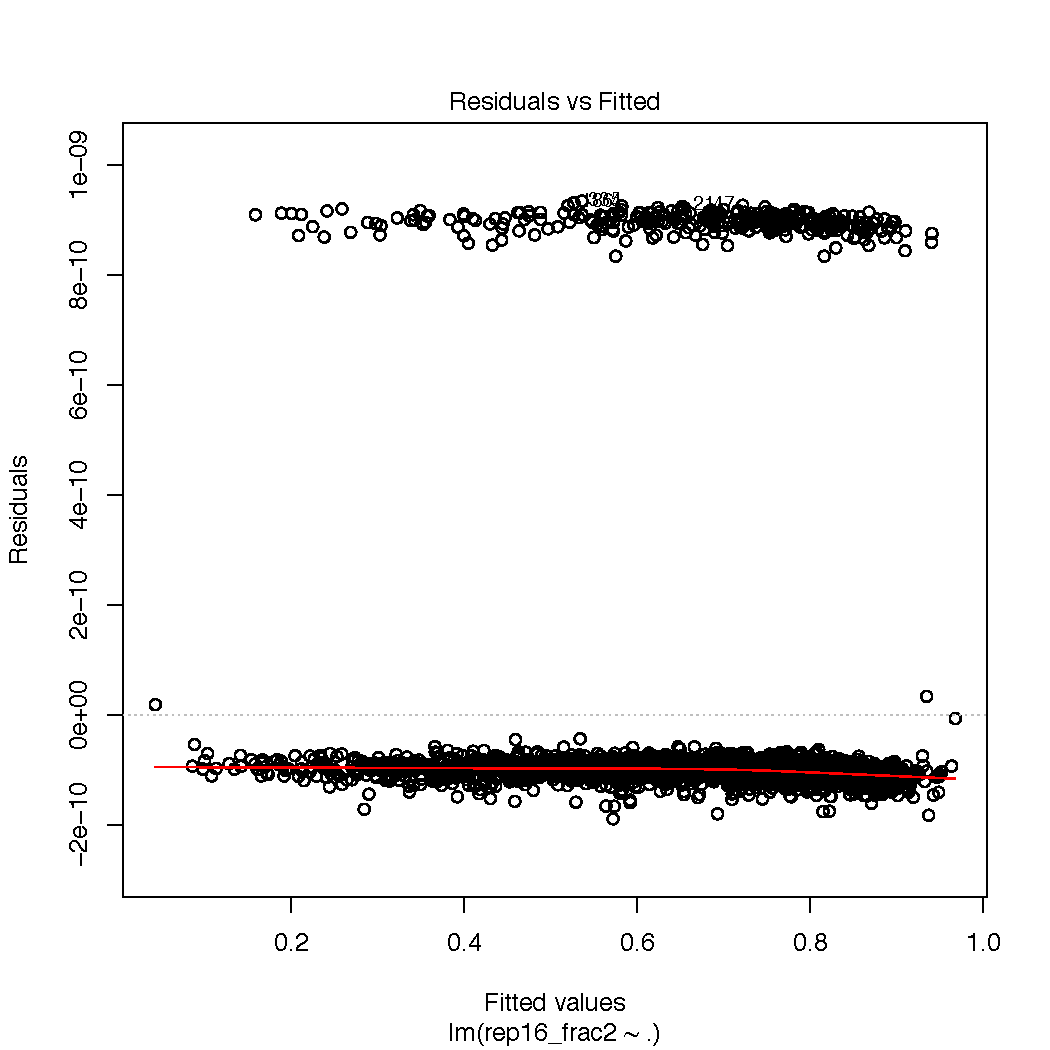
\includegraphics[width=.5\textwidth]{output_regression_Residuals}
	\caption{Residuals of the fitted outcome regression model}
    \label{outcome-regression}
\end{figure}

\section{Conclusion}
The contentious nature of the 2016 election, and politics and policy in general over the last 10 years has led to big shifts in public opinion. Few analysts thought Donald Trump was a reasonable contender to win the presidency, but won nonetheless. This paper aimed to look into what role the uninsured rate of counties played into his win. Using data at a county level from a variety of sources, including the New York Times, Measure of America, and the US Census, we used two methods of causal inference to study this. The first being a combination of inverse probability weighting and a quadratic structural model. We found that at the mean level, uninsured rate had an estimated marginal causal effect of ($0.1316 \pm 0.2643$). From this result, we can't conclude there is a causal effect on the outcome by the treatment at the mean value. The second method we used was outcome regression. In outcome regression we fit a linear model of the covariates and treatment to the mean value of the outcome given the covariates and treatment. Similar to our results for inverse probability weighting, we found that the mean causal effect of  $(-1.783708e-10\pm3.1705305e-10)$ contained the zero value within the confidence interval so we can't conclude the existence of any causal effect.

Although we weren't able to confirm any causal effects at the mean values of our outcome, our study still opens up some relevant questions and limitations relating to uninsured rate and political outlook. Our study looked at the rate of uninsured people roughly two years before the election. Future studies could benefit by looking at the change in insurance rate since the introduction of the Affordable Care Act as opposed as a time-varying treatment. This study is also limited in that we only study the fraction that are insured versus uninsured. In reality quality of insurance could differ drastically among different counties and even inside of one county. 

% trigger a \newpage just before the given reference
% number - used to balance the columns on the last page
% adjust value as needed - may need to be readjusted if
% the document is modified later
%\IEEEtriggeratref{8}
% The "triggered" command can be changed if desired:
%\IEEEtriggercmd{\enlargethispage{-5in}}

% references section

% can use a bibliography generated by BibTeX as a .bbl file
% BibTeX documentation can be easily obtained at:
% http://mirror.ctan.org/biblio/bibtex/contrib/doc/
% The IEEEtran BibTeX style support page is at:
% http://www.michaelshell.org/tex/ieeetran/bibtex/
%\bibliographystyle{IEEEtran}
% argument is your BibTeX string definitions and bibliography database(s)
%\bibliography{IEEEabrv,../bib/paper}
%
% <OR> manually copy in the resultant .bbl file
% set second argument of \begin to the number of references
% (used to reserve space for the reference number labels box)
\bibliographystyle{IEEEtran}
\bibliography{sample}

\end{document}


